% !TeX root = surprises.tex

\chapter{Solving Quadratic Equations}\label{c.quadratic}

%%%%%%%%%%%%%%%%%%%%%%%%%%%%%%%%%%%%%%%%%%%%%%%%%%%%%%%%%%%%%%%

\abstract*{This chapter presents Poh-Shen Loh method for solving quadratic equations that is based on a relation between the coefficients of the quadratic polynomial and its roots. Al-Khwarizmi's geometric solution of quadratic equations in presented along with Cardano's geometric construction used to development the formula for finding roots of cubic equations.}

%%%%%%%%%%%%%%%%%%%%%%%%%%%%%%%%%%%%%%%%%%%%%%%%%%%%%%%%%%%%%%%

Poh-Shen Loh\index{Loh, Poh-Shen} proposed a method for solving quadratic equations that is based on a relation between the coefficients of the quadratic polynomial and its roots. Section~\ref{s.traditional} reviews the traditional methods for solving quadratic equations. 
Section~\ref{s.computing} tries to convince the reader that Loh's method makes sense and then explains how to compute the roots. In Sect.~\ref{s.examples} the computation is carried out for two quadratic polynomials and a similar computation for a quartic polynomial. Section~\ref{s.general} derives the traditional formula for the roots from Loh's formulas.

The introduction of algebra and modern algebraic notation is relatively recent. Previously, mathematicians used geometry almost exclusively, so it is interesting to look at al-Khwarizmi's geometric construction of the formula for the roots of quadratic equations (Sect.~\ref{s.khwar}). Section~\ref{s.cardano} shows a clever geometric construct used by Cardano in developing the formula for the roots of cubic equations.

Section~\ref{s.lill-quadratic} presents other geometric methods for finding the roots of quadratic equations, but Chap.~\ref{c.origami-cube} is a prerequisite for a full understanding of these methods.

The chapter concludes with Sect.~\ref{s.numerical} which discusses numerical computation of roots of quadratic equations.

\section{Traditional Methods for Solving Quadratic Equations}\label{s.traditional}
\index{Quadratic equation}
Every student of mathematics memorizes the formula for obtaining the roots of a quadratic equation $ax^2+bx+c=0$:
\[
x_1, x_2 = \frac{-b\pm\sqrt{b^2-4ac}}{2a}\,.
\]                      
For now we will work only with monic\index{Monic polynomial}. The roots of $x^2+bx+c=0$ are:
\begin{align}
x_1, x_2 = \frac{-b\pm\sqrt{b^2-4c}}{2}\,.\label{eq.quadratic-roots}
\end{align}
Another method of solving quadratic equations is by factoring the polynomials more-or-less by trial-and-error. Sometimes it is easy to obtain the roots by factoring:
\begin{align}
x^2-4x+3= (x-1)(x-3)\label{eq.quadratic-lill}\,.
\end{align}


It is much harder to factor $x^2-2x-24$ because there are many possible pairs of roots that must be considered:
\[
(\pm 1,\mp 24)\,, (\pm 2,\mp 12)\,, (\pm 3,\mp 8)\,, (\pm 4,\mp 6)\,.
\]

\section{The Relation Between the Roots and the Coefficients}\label{s.computing}
\index{Quadratic equation!roots of}
\begin{theorem}\label{thm.roots-coefficients}
If $r_1,r_2$ are the roots of $x^2+bx+c$ then:
\[
(x-r_1)(x-r_2)=x^2 - (r_1+r_2)x + r_1r_2=x^2+bx+c\,.
\]
Therefore, even if we do not know the values of the roots, we do know that:
\begin{align}\label{eq.viete-quad}
r_1+r_2 = -b\,,\quad\quad r_1r_2=c\,.
\end{align}
\end{theorem}

There is really nothing to prove because the result emerges from the computation.

Consider some values of $-b,r_1,r_2$ and let $m_{12}$ be the average of $r_1,r_2$:
\[
\renewcommand{\arraystretch}{1.2}
\begin{array}{|@{\hspace{1em}}r|@{\hspace{1em}}r|@{\hspace{1em}}r|@{\hspace{1em}}r|}
\hline
-b& r_1 & r_2 &m_{12}\\\hline
33 & 12 & 21 & 16\frac{1}{2}\\\hline
33 & 8 & 25 & 16\frac{1}{2}\\\hline
33 & 1 & 32 & 16\frac{1}{2}\\\hline\hline
-b& r_1 & r_2 &m_{12}\\\hline
-4 & -16 & 12 & -2 \\\hline
-4 & -4 & 0 & -2 \\\hline
-4 & -3 & -1 & -2 \\\hline
\end{array}
\]

For any quadratic equation the average of the two roots is constant:
\[
m_{1,2}=\frac{r_1+r_2}{2}=
\frac{(-b-r_2)+r_2}{2}=
-\frac{b}{2}\,.
\]

\newpage

Let $s$ be any number. Then:
\[
-b=-b+s+(-s)=\left(\frac{-b}{2}+s\right) + \left(\frac{-b}{2}-s\right)=r_1+r_2\,.
\]
If one root is at distance $s$ from the average $m_{12}$, the other root is at distance $-s$ from  the average. For $r_1,r_2=2,6$, where $m_{12}=4, s=2$, we have:
\[
\renewcommand{\arraystretch}{1.2}
\begin{array}{|@{\hspace{1em}}r|@{\hspace{1em}}r|@{\hspace{1em}}r|@{\hspace{1em}}r|r|r|}
\hline
-b& r_1 & r_2 & m_{12}& m_{12}\!-\!r_1 & m_{12}\!-\!r_2\\\hline
33 & 12 & 21 & 16\frac{1}{2}&4\frac{1}{2} & -4\frac{1}{2}  \\\hline
33 & 8 & 25 & 16\frac{1}{2}&8\frac{1}{2}&-8\frac{1}{2}\\\hline
33 & 1 & 32 & 16\frac{1}{2}&15\frac{1}{2}&-15\frac{1}{2}\\\hline
\hline
-4 & -16 & 12 & -2 &14& -14\\\hline
-4 & -4 & 0 & -2&2&-2 \\\hline
-4 & -3 & -1 & -2&1&-1 \\\hline
\end{array}
\]
Figure~\ref{f.loh-roots1} visualizes this relation.
\begin{figure}[t]
\begin{center}
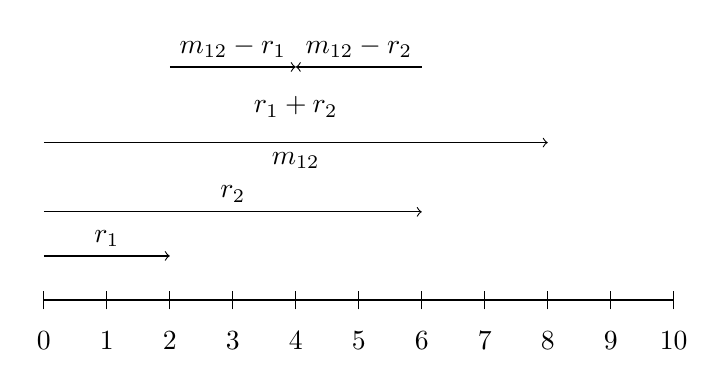
\begin{tikzpicture}[scale=.8]
\begin{scope}[yshift=-4mm]
\draw (0,0) -- (10,0);
\foreach \x in {0,1,...,10}
  \draw (\x,-1.5mm) -- +(0,3mm) node[below,yshift=-4mm] {$\x$};
\draw[->,yshift=7mm] (0,0) -- node[above] {$r_1$} (20mm,0);
\draw[->,yshift=14mm] (0,0) -- node[above] {$r_2$} (60mm,0);
\end{scope}
\draw[->,yshift=21mm] (0,0) -- node[above,yshift=2mm] {$r_1+r_2$} (80mm,0);
\coordinate (M) at (40mm,21mm);
\vertex{M};
\node[below] at (40mm,21mm) {$m_{12}$};
\begin{scope}[yshift=3mm]
\draw[->,yshift=30mm] (20mm,0mm) -- node[above] {$m_{12}-r_1$} +(20mm,0);
\draw[->,yshift=30mm] (60mm,0mm) -- node[above] {$m_{12}-r_2$} +(-20mm,0);
\end{scope}
\end{tikzpicture}
\end{center}
\caption{Relation between the roots $r_1,r_2=2,6$ and their average $m_{12}=4$}
\label{f.loh-roots1}
\end{figure}
If we use other values $r_1,r_2=3,5$ for which $r_1+r_2=8$, then $m_{12}=4$ remains the same while $s$ becomes $1$ (Fig.~\ref{f.loh-roots2}).
\begin{figure}[b]
\begin{center}
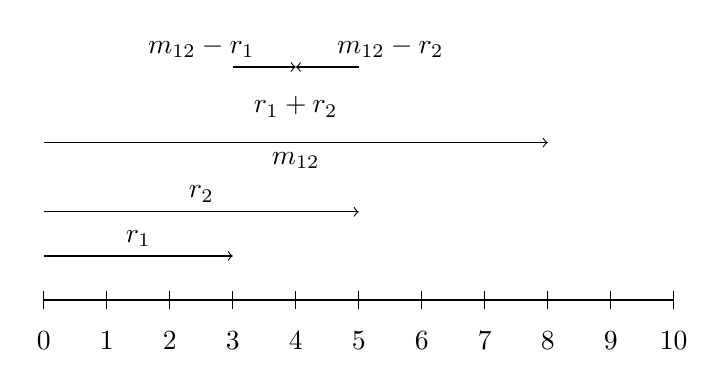
\begin{tikzpicture}[scale=.8]
\begin{scope}[yshift=-4mm]
\draw (0,0) -- (10,0);
\foreach \x in {0,1,...,10}
  \draw (\x,-1.5mm) -- +(0,3mm) node[below,yshift=-4mm] {$\x$};
\draw[->,yshift=7mm] (0,0) -- node[above] {$r_1$} (30mm,0);
\draw[->,yshift=14mm] (0,0) -- node[above] {$r_2$} (50mm,0);
\end{scope}
\draw[->,yshift=21mm] (0,0) -- node[above,yshift=2mm] {$r_1+r_2$}(80mm,0);
\coordinate (M) at (40mm,21mm);
\vertex{M};
\node[below] at (40mm,21mm) {$m_{12}$};
\begin{scope}[yshift=3mm]
\draw[->,yshift=30mm] (30mm,0mm) -- node[above left] {$m_{12}-r_1$} +(10mm,0);
\draw[->,yshift=30mm] (50mm,0mm) -- node[above right] {$m_{12}-r_2$} +(-10mm,0);
\end{scope}
\end{tikzpicture}
\end{center}
\caption{Relation between the roots $r_1,r_2=3,5$ and their average $m_{12}=4$}
\label{f.loh-roots2}
\end{figure}
The offset $s$ seems to be arbitrary in:
\[
r_1=\left(\frac{-b}{2}+s\right)\,,\quad r_2=\left(\frac{-b}{2}-s\right)\,,
\]
\enlargethispage{\baselineskip}
\hspace*{-4pt}but there is an additional constraint $r_1r_2=c$, where $c$ is the constant term in the polynomial.
By multiplying the two expressions we have derived for $r_1,r_2$, we can determine $s$ and then $r_1,r_2$:
\[
c=\left(-\frac{b}{2} +s\right)\left(-\frac{b}{2} -s\right)\,.
\]

\section{Examples of Loh's Method}\label{s.examples}

\begin{example}
Consider the polynomial  $x^2-2x-24$, where $b=-2,c=-24$:
\begin{eqnarray*}
c&=&\left(-\frac{(-2)}{2} +s\right)\left(-\frac{(-2)}{2} -s\right)\\
-24&=&(1 +s)(1 -s)\\
%s^2&=&25\\
s&=&5\\
r_1&=&1+5=6\\
r_2&=&1-5=-4\,.
\end{eqnarray*}
Check: $(x-6)(x-(-4))= x^2-2x-24$.
\end{example}

\begin{example}
Let us find the roots of $x^2-83x-2310$:
\begin{eqnarray*}
%c&=&\left(-\frac{b}{2} +s\right)\left(-\frac{b}{2} -s\right)\\
-2310&=&\left(\frac{83}{2}+s\right)\left(\frac{83}{2} -s\right)\\
s^2&=&\frac{6889}{4}+2310=\frac{16129}{4}\\
s&=&\frac{127}{2}\\
r_1&=&\frac{83}{2}-\frac{127}{2}=-22\\
r_2&=&\frac{83}{2}+\frac{127}{2}=105\,.
\end{eqnarray*}
Check: $(x+22)(x-105)= x^2-83x-2310$.

\newpage

Compare this computation with the computation using the traditional  formula:
\begin{eqnarray*}
\frac{-b\pm\sqrt{b^2-4c}}{2}&=&\frac{-(-83)\pm\sqrt{(-83)^2-4\cdot (-2310)}}{2}\\
%&=& \frac{83\pm\sqrt{6889+9240}}{2} = \frac{83\pm\sqrt{16129}}{2}\\
&=& \frac{83\pm\sqrt{16129}}{2} = \frac{83\pm 127}{2}\\
r_1&=&\frac{83-127}{2}=-22\\
r_2&=&\frac{83+127}{2}=105\,.
\end{eqnarray*}
\end{example}

\begin{example}
Theorem~\ref{thm.roots-coefficients} can be generalized to polynomials of higher degrees. Here is an interesting example for a \emph{quartic equation}\index{Quartic equation} $x^4-10x^2-x+20=0$. As with quadratic equations, there are formulas for solving cubic and quartic equations (though not equations of higher powers), but the formulas are quite complicated.

Does this polynomial of degree four factor into two quadratic polynomials with integer coefficients? \textit{If so, the coefficients of the $x$ terms must be equal and of opposite signs, since the coefficient of the $x^3$ term is zero!} Therefore, the form of the quadratic factors is:
\[
f(x) = (x^2 - nx + k_1)\, (x^2 + nx + k_2)\,.
\]
Carrying out the multiplication results in:
\[
\renewcommand{\arraystretch}{1.1}
\begin{array}{rrrrrr}
f(x) = &x^4 & + nx^3 & + k_2 x^2\\
&& -nx^3 &- n^2x^2 &-nk_2x\\
&&&+k_1x^2 &+ nk_1x &+ k_1k_2\,.
\end{array}
\]
Equating the coefficients gives three equations in the three unknowns $n,k_1,k_2$:
\begin{eqnarray*}
(k_1+k_2)-n^2 &=& -10\\
n(k_1-k_2) &=& -1\\
k_1k_2 &=& 20\,.
\end{eqnarray*}
Since we are looking for factors with integer coefficients, from the last two equations it is clear that:
\[
n=1,\,k_1=4,\,k_2=5  \quad\quad\textrm{or} \quad\quad n=1,\,k_1=-5,\, k_2=-4\,.
\]
Only $n=1,k_1=-5,\, k_2=-4$ satisfy the first equation for the coefficient of $x^2$:
\[
f(x) = (x^2 - x - 5)\, (x^2 + x - 4)\,.
\]

\newpage

Solving these quadratic equations gives four solutions of the quartic equation:
\[
x = \frac{1\pm\sqrt{21}}{2}  \;\;\textrm{or} \;\; x= \frac{-1\pm\sqrt{17}}{2} \,.
\]
\end{example}

\section{Derivation of the Traditional Formula}\label{s.general}
\index{Quadratic equation!traditional formula}
For an arbitrary monic polynomial $x^2+bx+c$, Loh's formulas are:
\begin{eqnarray*}
c=r_1r_2&=&\left(\frac{-b}{2}+s\right)  \left(\frac{-b}{2}-s\right)=\left(\frac{b^2}{4}-s^2\right)\\
s&=&\sqrt{\left(\frac{b^2}{4}\right)-c}\\
r_1,r_2&=&\frac{-b}{2}\pm\sqrt{\left(\frac{b^2}{4}\right)-c}=\frac{-b\pm\sqrt{b^2-4c}}{2}\,,
\end{eqnarray*}
the traditional formula for obtaining the roots of a monic\index{Monic polynomial} quadratic polynomial. If the polynomial is not monic divide it by $a$, substitute in the  equation and simplify:
\begin{eqnarray*}
%ax^2+bx+c&=&0\\
x^2+\frac{b}{a}x+\frac{c}{a}&=&0\\
r_1,r_2&=&\frac{-(b/a)\pm\sqrt{(b/a)^2-4(c/a)}}{2}\\
%&=&\frac{-(b/a)\pm\sqrt{(b/a)^2-4(ac/a^2)}}{2}\\
&=&\frac{-b\pm\sqrt{b^2-4ac}}{2a}\,.
\end{eqnarray*}

\section{Al-Khwarizmi's Geometric Solution of Quadratic Equations}\label{s.khwar}

Let us write a monic\index{Monic polynomial} quadratic polynomial as $x^2+bx-c$. The roots can be found by \emph{completing the square}\index{Quadratic equation!completing the square}:
\begin{eqnarray*}
%x^2+bx&=&c\\
x^2+2\left(\frac{b}{2}\right)x+\left(\frac{b}{2}\right)^2&=&c+\left(\frac{b}{2}\right)^2\\
\left(x+\frac{b}{2}\right)^2&=&c+\left(\frac{b}{2}\right)^2\\
x&=&-\frac{b}{2}\pm\sqrt{c+\left(\frac{b}{2}\right)^2}=
\frac{-b\pm\sqrt{b^2+4c}}{2}\,.
\end{eqnarray*}
This is the familiar formula for finding the roots of a quadratic equation, except that $4c$ has the opposite sign since the  coefficient of the constant term was $-c$.

Completing the square was developed in the $8$th century by Muhammad ibn Musa al-Khwarizmi in a geometric context. Given the equation $x^2+bx=c$, assume that there is a square whose side is 
$x$ so that its area is $x^2$.
To the area $x^2$ add $bx$ by adding four rectangles of area $bx/4$ whose sides are $b/4$ and $x$ (Fig.~\ref{f.khw-1}). Now complete the diagram to a square by adding the four little squares of area $(b/4)^2$ (Fig.~\ref{f.khw-2}).

\begin{figure}[b]
\subfigures
\leftfigure[c]{
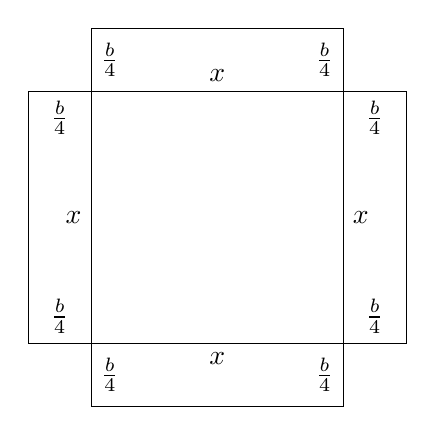
\begin{tikzpicture}[scale=.8]
\coordinate (A) at (0,0);
\coordinate (B) at (4,0);
\coordinate (C) at (4,4);
\coordinate (D) at (0,4);
\draw (A) -- node[below] {$x$} (B) -- node[right] {$x$} (C) -- node[above] {$x$} (D) -- node[left] {$x$} cycle;
\draw (A) -- node[right] {$\frac{b}{4}$} ++(0,-1) -- ++(4,0) -- node[left] {$\frac{b}{4}$} ++(0,1);
\draw (B) -- node[above] {$\frac{b}{4}$} ++(1,0) -- ++(0,4) -- node[below] {$\frac{b}{4}$} ++(-1,0);
\draw (C) -- node[left] {$\frac{b}{4}$} ++(0,1) -- ++(-4,0) -- node[right] {$\frac{b}{4}$} ++(0,-1);
\draw (D) -- node[below] {$\frac{b}{4}$} ++(-1,0) -- ++(0,-4) -- node[above] {$\frac{b}{4}$} ++(1,0);
\end{tikzpicture}
}
\hfill
\rightfigure[c]{
\begin{tikzpicture}[scale=.8]
\coordinate (A) at (0,0);
\coordinate (B) at (4,0);
\coordinate (C) at (4,4);
\coordinate (D) at (0,4);
\draw (A) -- node[below] {$x$} (B) -- node[right] {$x$} (C) -- node[above] {$x$} (D) -- node[left] {$x$} cycle;
\draw (A) -- node[right] {$\frac{b}{4}$} ++(0,-1) -- ++(4,0) -- node[left] {$\frac{b}{4}$} ++(0,1);
\draw (B) -- node[above] {$\frac{b}{4}$} ++(1,0) -- ++(0,4) -- node[below] {$\frac{b}{4}$} ++(-1,0);
\draw (C) -- node[left] {$\frac{b}{4}$} ++(0,1) -- ++(-4,0) -- node[right] {$\frac{b}{4}$} ++(0,-1);
\draw (D) -- node[below] {$\frac{b}{4}$} ++(-1,0) -- ++(0,-4) -- node[above] {$\frac{b}{4}$} ++(1,0);
\draw[thick,dashed] ($(A)+(0,-1)$) -- ++(-1,0) -- ++(0,1);
\draw[thick,dashed] ($(B)+(0,-1)$) -- ++(1,0) -- ++(0,1);
\draw[thick,dashed] ($(C)+(0,1)$) -- ++(1,0) -- ++(0,-1);
\draw[thick,dashed] ($(D)+(0,1)$) -- ++(-1,0) -- ++(0,-1);
\end{tikzpicture}
}
\leftcaption{The area is $x^2+4(b/4)x=x^2+bx$}\label{f.khw-1}
\rightcaption{The area is $x^2+4(b/4)x+4(b/4)^2=x^2+bx+(b^2/4)$}\label{f.khw-2}
\end{figure}

We can't construct the diagram in Fig.~\ref{f.khw-1} because we don't know what $x$ is, but the area of the larger square in  Fig.~\ref{f.khw-2} is:
\[
x^2+bx+\frac{b^2}{4}=c+\frac{b^2}{4}\,,
\]
which we do know since we are given the coefficients $b,c$. By constructing the diagram and erasing the small squares whose sides are $(b/4)$---another known quantity---we obtain the line segment of length $x$.

\begin{example}
Let $x^2+12x=64$. Then $c+(b^2/4)=64+36=100$. It is easy to construct a square of area $100$ since each side has length $10$. Now subtract $(b/4)+(b/4)=6$, the sides of the smaller squares, to get $x=10-6=4$.
\end{example}

\section{Cardano's Construction for Solving Cubic Equations}\label{s.cardano}

The formula for the roots of cubic equations\index{Cubic equation} was first published in the $16$th century by Gerolamo Cardano\index{Cardano, Gerolamo}. We will not develop the formula here, but it is interesting that the central idea is based on a geometric construction similar to al-Khwarizmi's. The construction can be obtained very simply using algebra. By multiplication:
\begin{align}\label{eq.car}
(a+b)^3=a^3+3a^2b+3ab^2+b^3=(a^3+b^3)+3ab(a+b)\,.
\end{align}
Geometrically, we start with a cube whose side is $a+b$ so that its volume is $(a+b)^3$. The cube is decomposed into five pieces. The first two are cubes whose sides are $a$ and $b$ with volumes $a^3$ (blue) and $b^3$ (red), respectively (Fig.~\ref{f.cardano1}).

The other three parts are boxes,\footnote{The technical term is \emph{cuboid}.} each with one side of length $a+b$ coinciding with a side of the cube, one side of length $a$ and one side of length $b$, so that the volume of each of the three boxes is $ab(a+b)$. In Fig.~\ref{f.cardano2}, there is one box at the left side of the cube (blue), one at the back of the cube (red) and one at the top of the cube (green).
By combining the five solids in Fig.~\ref{f.cardano1} and Fig.~\ref{f.cardano2} we obtain Eq.~\ref{eq.car}.


\begin{figure}[htb]
\begin{center}
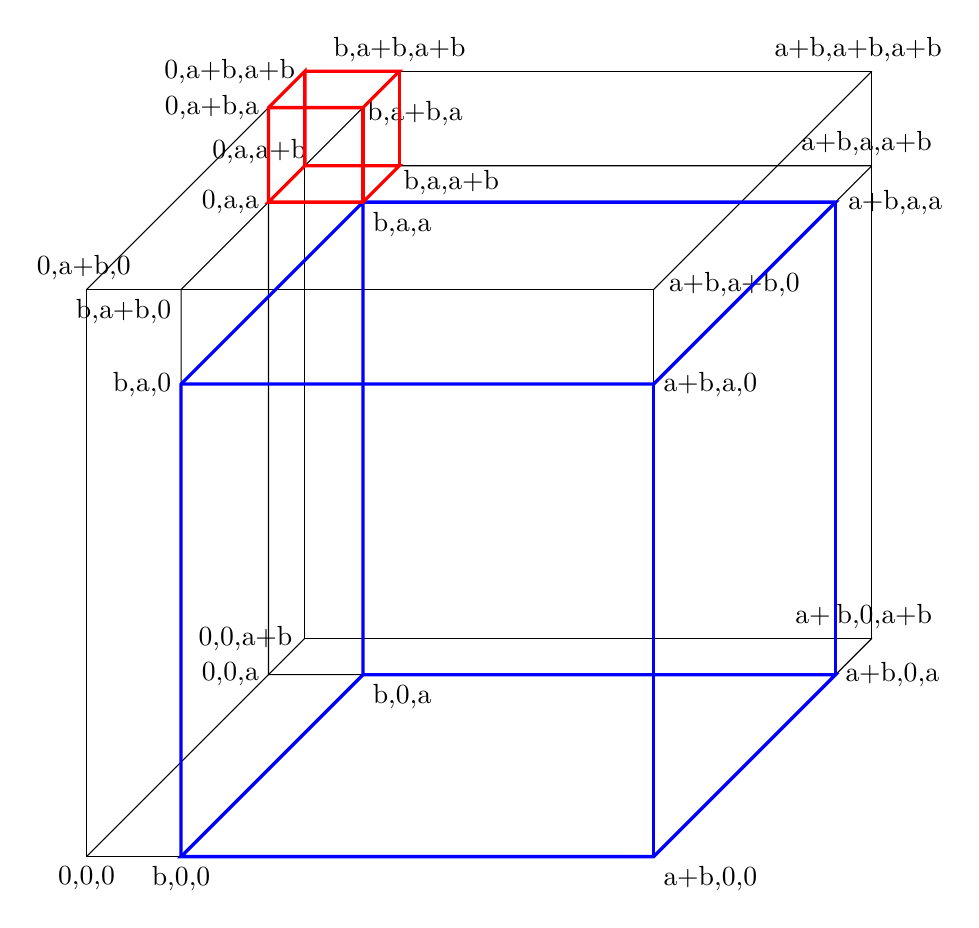
\begin{tikzpicture}[scale=1.2]

% Front face
\coordinate (A) at (0,0,0);
\node[below] at (A) {\sm{0,0,0}};
\coordinate (B) at (6,0,0);
\node[below right] at (B) {\sm{a+b,0,0}};
\coordinate (C) at (6,6,0);
\node[above right,xshift=2pt,yshift=-6pt] at (C)
  {\sm{a+b,a+b,0}};
\coordinate (D) at (0,6,0);
\node[above,xshift=-1pt] at (D) {\sm{0,a+b,0}};

% Front face
\coordinate (FF1) at (1,0,0);
\node[below] at (FF1) {\sm{b,0,0}};
\coordinate (FF2) at (1,5,0);
\node[left] at (FF2) {\sm{b,a,0}};
\coordinate (FF3) at (1,6,0);
\node[below left] at (FF3) {\sm{b,a+b,0}};
\coordinate (FF4) at (6,5,0);
\node[right] at (FF4) {\sm{a+b,a,0}};

% Back face
\coordinate (A1) at (0,0,-6);
\node[left,xshift=-1pt] at (A1) {\sm{0,0,a+b}};
\coordinate (B1) at (6,0,-6);
\node[above,xshift=-3pt] at (B1) {\sm{a+\:b,0,a+b}};
\coordinate (C1) at (6,6,-6);
\node[above,xshift=-5pt] at (C1) {\sm{a+b,a+b,a+b}};
\coordinate (D1) at (0,6,-6);
\node[left] at (D1) {\sm{0,a+b,a+b}};

% Back face
\coordinate (BF1) at (0,5,-6);
\node[above left,xshift=4pt,yshift=-3pt] at (BF1) 
  {\sm{0,a,a+b}};
\coordinate (BF2) at (1,5,-6);
\node[below right,xshift=-2pt,yshift=2pt] at (BF2)
  {\sm{b,a,a+b}};
\coordinate (BF3) at (1,6,-6);
\node[above] at (BF3) {\sm{b,a+b,a+b}};
\coordinate (BF4) at (6,5,-6);
\node[above,xshift=-2pt] at (BF4) {\sm{a+b,a,a+b}};

% Right face
\coordinate (RF1) at (6,5,-5);
\node[right,xshift=1pt] at (RF1) {\sm{a+b,a,a}};
\coordinate (RF2) at (6,0,-5);
\node[right] at (RF2) {\sm{a+b,0,a}};

% Bottom face
\coordinate (BT1) at (1,0,-5);
\node[below right] at (BT1) {\sm{b,0,a}};

% Left face
\coordinate (LF1) at (0,0,-5);
\node[left] at (LF1) {\sm{0,0,a}};
\coordinate (LF2) at (0,5,-5);
\node[left] at (LF2) {\sm{0,a,a}};
\coordinate (LF3) at (0,6,-5);
\node[left] at (LF3) {\sm{0,a+b,a}};

% Top face
\coordinate (TF1) at (1,6,-5);
\node[right,xshift=-2pt,yshift=-2pt] at (TF1) {\sm{b,a+b,a}};

% Internal point
\coordinate (I) at (1,5,-5);
\node[below right] at (I) {\sm{b,a,a}};


\draw (A) -- (B) -- (C) -- (D) -- cycle;
\draw (A1) -- (B1) -- (C1) -- (D1) -- cycle;
\draw (A) -- (A1);
\draw (B) -- (B1);
\draw (C) -- (C1);
\draw (D) -- (D1);

\draw (FF1) -- (FF2) -- (FF3) -- (BF3);
\draw (BF2) -- (FF2) -- (FF4) -- (BF4);
\draw (FF1) -- (BT1) -- (TF1);
\draw (BF3) -- (BF2);
\draw (TF1) -- (LF3);
\draw (LF3) -- (LF1) -- (RF2) -- (RF1) -- (LF2) -- 
      (BF1) -- (BF4);

\draw[very thick,blue] (FF1) -- (B) -- (RF2) -- (BT1) -- cycle; 
\draw[very thick,blue] (FF1) -- (FF2) -- (I) -- (BT1);
\draw[very thick,blue] (I) -- (RF1) -- (FF4) -- (FF2);
\draw[very thick,blue] (FF4) -- (B);
\draw[very thick,blue] (RF1) -- (RF2);

\draw[very thick,red] (I) -- (LF2) -- (BF1) -- (BF2) -- cycle;
\draw[very thick,red] (LF2) -- (LF3) -- (D1) -- (BF1);
\draw[very thick,red] (D1) -- (BF3) -- (TF1) -- (LF3);
\draw[very thick,red] (TF1) -- (I);
\draw[very thick,red] (BF3) -- (BF2);

\end{tikzpicture}
\end{center}
\caption{$(a^3+b^3)=(a^3+b^3)+\cdots$}\label{f.cardano1}
\end{figure}

%%%%%%%%%%%%%%%%%%%%%%%%%%%%%%%%%%%%%%%%%%%%%%%%%%%%%%%%%%%%%

\begin{figure}[htb]
\begin{center}
\begin{tikzpicture}[scale=1.2]

% Front face
\coordinate (A) at (0,0,0);
\node[below] at (A) {\sm{0,0,0}};
\coordinate (B) at (6,0,0);
\node[below right] at (B) {\sm{a+b,0,0}};
\coordinate (C) at (6,6,0);
\node[above right,xshift=2pt,yshift=-6pt] at (C)
  {\sm{a+b,a+b,0}};
\coordinate (D) at (0,6,0);
\node[above,xshift=-1pt] at (D) {\sm{0,a+b,0}};

% Front face
\coordinate (FF1) at (1,0,0);
\node[below] at (FF1) {\sm{b,0,0}};
\coordinate (FF2) at (1,5,0);
\node[left] at (FF2) {\sm{b,a,0}};
\coordinate (FF3) at (1,6,0);
\node[below left] at (FF3) {\sm{b,a+b,0}};
\coordinate (FF4) at (6,5,0);
\node[right] at (FF4) {\sm{a+b,a,0}};

% Back face
\coordinate (A1) at (0,0,-6);
\node[left,xshift=-1pt] at (A1) {\sm{0,0,a+b}};
\coordinate (B1) at (6,0,-6);
\node[above,xshift=-3pt] at (B1) {\sm{a+\:b,0,a+b}};
\coordinate (C1) at (6,6,-6);
\node[above,xshift=-5pt] at (C1) {\sm{a+b,a+b,a+b}};
\coordinate (D1) at (0,6,-6);
\node[left] at (D1) {\sm{0,a+b,a+b}};

% Back face
\coordinate (BF1) at (0,5,-6);
\node[above left,xshift=4pt,yshift=-3pt] at (BF1) 
  {\sm{0,a,a+b}};
\coordinate (BF2) at (1,5,-6);
\node[below right,xshift=-2pt,yshift=2pt] at (BF2)
  {\sm{b,a,a+b}};
\coordinate (BF3) at (1,6,-6);
\node[above] at (BF3) {\sm{b,a+b,a+b}};
\coordinate (BF4) at (6,5,-6);
\node[above,xshift=-2pt] at (BF4) {\sm{a+b,a,a+b}};

% Right face
\coordinate (RF1) at (6,5,-5);
\node[right,xshift=1pt] at (RF1) {\sm{a+b,a,a}};
\coordinate (RF2) at (6,0,-5);
\node[right] at (RF2) {\sm{a+b,0,a}};

% Bottom face
\coordinate (BT1) at (1,0,-5);
\node[below right] at (BT1) {\sm{b,0,a}};

% Left face
\coordinate (LF1) at (0,0,-5);
\node[left] at (LF1) {\sm{0,0,a}};
\coordinate (LF2) at (0,5,-5);
\node[left] at (LF2) {\sm{0,a,a}};
\coordinate (LF3) at (0,6,-5);
\node[left] at (LF3) {\sm{0,a+b,a}};

% Top face
\coordinate (TF1) at (1,6,-5);
\node[right,xshift=-2pt,yshift=-2pt] at (TF1) {\sm{b,a+b,a}};

% Internal point
\coordinate (I) at (1,5,-5);
\node[below right] at (I) {\sm{b,a,a}};


\draw (A) -- (B) -- (C) -- (D) -- cycle;
\draw (A1) -- (B1) -- (C1) -- (D1) -- cycle;
\draw (A) -- (A1);
\draw (B) -- (B1);
\draw (C) -- (C1);
\draw (D) -- (D1);

\draw (FF1) -- (FF2) -- (FF3) -- (BF3);
\draw (BF2) -- (FF2) -- (FF4) -- (BF4);
\draw (FF1) -- (BT1) -- (TF1);
\draw (BF3) -- (BF2);
\draw (TF1) -- (LF3);
\draw (LF3) -- (LF1) -- (RF2) -- (RF1) -- (LF2) -- 
      (BF1) -- (BF4);

\draw[very thick,blue] (A) -- (FF1) -- (FF3) -- (D) -- cycle;
\draw[very thick,blue] (FF1) -- (BT1) -- (TF1) -- (FF3);
\draw[very thick,blue] (TF1) -- (LF3) -- (D);
\draw[very thick,blue] (LF3) -- (LF1) -- (A);
\draw[very thick,blue] (LF1) -- (BT1);

\draw[very thick,red] (LF1) -- (RF2) -- (RF1) -- (LF2);
\draw[very thick,red] ($(LF2) + (2pt,0)$) -- ($(LF1) + (2pt,0)$);
\draw[very thick,red] (A1) -- (B1) -- (BF4) -- (BF1) -- cycle;
\draw[very thick,red] ($(LF2) + (2pt,0)$) -- ($(BF1) + (2pt,0)$);
\draw[very thick,red] (BF4) -- (RF1);
\draw[very thick,red] (B1) -- (RF2);
\draw[very thick,red] (A1) -- (LF1);

\draw[very thick,green] (FF2) -- (FF4) -- (C) -- (FF3);
\draw[very thick,green] 
  ($(FF2) + (2pt,0)$) -- ($(FF3) + (2pt,0)$);
\draw[very thick,green] 
  ($(FF4) + (0,2pt)$) -- ($(BF4) + (0,2pt)$);
\draw[very thick,green] (BF4) -- (C1) -- (BF3);
\draw[very thick,green] 
  ($(BF3) + (2pt,0)$) -- ($(FF3) + (2pt,0)$);
\draw[very thick,green] (C1) -- (C);
\draw[very thick,green] (BF3) -- (BF2) -- (FF2);
\draw[very thick,green] 
  ($(BF2) + (0,2pt)$) -- ($(BF4) + (0,2pt)$);


\end{tikzpicture}
\end{center}
\caption{$(a^3+b^3)=\cdots+3ab(a+b)$}\label{f.cardano2}
\end{figure}

\section{They Weren't Intimidated by Imaginary Numbers}\label{s.imaginary}

The history of mathematics demonstrates a progression of concepts that were initially considered to be meaningless, but were eventually understood, accepted and proved useful. ``Obviously,'' since numbers count things, $-1$, a negative number, is meaningless. ``Obviously,'' since numbers are ratios of integers (rational numbers), $\sqrt{2}$, which can easily be proved to be irrational, is meaningless. ``Obviously,'' $\sqrt{-1}$, the square root of a negative number, is meaningless since there is no number---integer, rational or even real---whose square is $-1$.

A full understanding of the square roots of negative numbers, to this day called \emph{imaginary numbers} although they are no less real than real numbers, was not achieved until the nineteenth century. Therefore, it is surprising that already in the sixteenth century, Geralamo Cardano and Rafael Bombelli refused to be intimidated by the concept, and took the first small steps towards understanding these numbers.

Consider the quadratic equation:
\begin{align}
x^2-10x+40=0\,.\label{eq.cardano-quadratic}
\end{align}
By the familiar formula (Eq.~\ref{eq.quadratic-roots}):
\[
r_1, r_2=\displaystyle\frac{10\pm\sqrt{100-160}}{2}=5\pm\sqrt{-15}\,.
\]
Well, we don't know anything about the square roots of negative numbers and we don't know what these values are, but like Cardano we do know by Thm~\ref{eq.quadratic-roots} that:
\[
\begin{array}{lcl}
r_1+r_2&=&(5+\sqrt{-15})+(5-\sqrt{-15})=10=-b\\
r_1r_2&=&(5+\sqrt{-15})(5-\sqrt{-15})=25-5\sqrt{-15}+5\sqrt{-15}-(-15)=40=c\,.
\end{array}
\]
which correspond with the coefficients of the quadratic equation Eq.~\ref{eq.cardano-quadratic}. It is rather intuitive that $a+(-a)=0$ even if we know nothing about $a$ and $-a$, and, similarly, it is rather intuitive that $\sqrt{a}\sqrt{a}=a$ even if we don't know what $\sqrt{a},\sqrt{-a}$ are.

\enlargethispage{\baselineskip}

Consider now the cubic equation:
\begin{align}
x^3-15x-4=0\,.\label{eq.bombelli-cubic}
\end{align}
It is not hard to observe that $4$ is a root, but how can it be computed? Cardano's formula gives the root:
\begin{align}
r=\sqrt[3]{2+11\sqrt{-1}}+\sqrt[3]{2-11\sqrt{-1}}\,,\label{eq.cube-root}
\end{align}
a quite complicated formula that bears no obviously relation to $4$. 

Bombelli courageously performed the following computation (see Eq.~\ref{eq.car}):
\begin{eqnarray*}
(2+\sqrt{-1})^3&=&
8+3\cdot 4\sqrt{-1}+3\cdot 2(-1)+(-1\sqrt{-1})=
2+11\sqrt{-1}\\
(2-\sqrt{-1})^3&=&
8-3\cdot 4\sqrt{-1}+3\cdot 2(-1)-(-1\sqrt{-1})=
2-11\sqrt{-1}\,,
\end{eqnarray*}
and by Eq.~\ref{eq.cube-root}:
\begin{eqnarray*}
r&=&\sqrt[3]{2+11\sqrt{-1}} + \sqrt[3]{2-11\sqrt{-1}}\\
&=&\sqrt[3]{(2+\sqrt{-1})^3} + \sqrt[3]{(2-\sqrt{-1})^3}\\
&=&(2+\sqrt{-1}) + (2-\sqrt{-1})=4\,.
\end{eqnarray*}


%%%%%%%%%%%%%%%%%%%%%%%%%%%%%%%%%%%%%%%%%%%%%%%%%%%%%%%%

\section{Lill's Method and Carlyle's Circle}\label{s.lill-quadratic}

Lill's method can be applied to solve quadratic equations.\footnote{This section assumes that you have read about Lill's method in Chap.~\ref{c.origami-cube}.}\index{Lill's method!quadratic equations} As an example we use Eq.~\ref{eq.quadratic-lill} which gives the roots of a quadratic equation obtained by factorization:
\[
x^2+bx+c=x^2-4x+3= (x-1)(x-3)\,.
\]
Applying Lill's method results in the paths shown in Fig.~\ref{f.lill-quadratic}.

\begin{figure}[bt]
\begin{center}
\begin{tikzpicture}[scale=1.1]
% Draw help lines and axes
\draw[step=10mm,white!50!black] (-4,-5) grid (2,1);
\draw[thick] (-4,0) -- (2,0);
\draw[thick] (0,-5) -- (0,1);
\foreach \x in {-3,...,2}
  \node at (\x-.2,.2) {\sm{\x}};
\foreach \y in {-4,...,-1}
  \node at (-.2,\y-.3) {\sm{\y}};

 Draw first path
\coordinate (A) at (0,0);
\coordinate (B) at (1,0);
\coordinate (C) at (1,-4);
\coordinate (D) at (-2,-4);
\draw[very thick] (A) --
  node[above] {$1$} (B);
\draw[very thick,name path=bc] (B) -- 
  node[right,xshift=-1pt,yshift=6pt] {$b=-4$} (C);
\draw[very thick,name path=cd] (C) --
  node[below left,xshift=3pt] {$c=3$}(D);

% Draw first segment of second path
\path[name path=a2] (A) -- +(-45:1.414);
\path [name intersections = {of = a2 and bc, by = {A2}}];
\node[above right] at (A2) {$P_1$};
\draw[very thick,dashed] (A) -- (A2);
\draw ($(A) + (14pt,0)$)
  arc [start angle=0, end angle = -45, radius=14pt];
\node[below right,xshift=40pt,yshift=-2pt] at (A) {$-45^\circ$};
\draw[->] ($(A)+(33pt,-6pt)$) -- +(-18pt,0);
\draw[rotate=135] (A2) rectangle +(5pt,5pt);

% Draw second segment of second path
\path[name path=b2] (A2) -- +(-135:5);
\path [name intersections = {of = b2 and cd, by = {B2}}];
\draw[very thick,dashed] (A2) -- (B2);

% Draw first segment of second path
\path[name path=a3] (A) -- +(-71.57:4);
\path [name intersections = {of = a3 and bc, by = {A3}}];
\node[above right] at (A3) {$P_2$};
\draw[very thick,dashed] (A) -- (A3);
\draw ($(A) + (20pt,0)$)
  arc [start angle=0, end angle = -71.57, radius=20pt];
\node[below right,xshift=40pt,yshift=-10pt] at (A) {$-71.57^\circ$};
\draw[->] ($(A)+(35pt,-13pt)$) -- +(-18pt,0);
\draw[rotate=108.43] (A3) rectangle +(5pt,5pt);

% Draw second segment of second path
\path[name path=b3] (A3) -- +(198.43:5);
\path [name intersections = {of = b3 and cd, by = {B3}}];
\draw[very thick,dashed] (A3) -- (B3);

\end{tikzpicture}
\end{center}
\caption{Lill's method on $x^2-4x+3$}\label{f.lill-quadratic}
\end{figure}
Check that the angles are correct:
\[
-\tan (-45^\circ) = -1,\quad -\tan (-71.57^\circ) \approx -3\,.
\]
For quadratic equations we can find the points $P_1,P_2$ as the intersections of the line representing the coefficient $b$ and the circle whose diameter is the line connecting the starting point and the end point of the paths (Fig.~\ref{f.lill-circle}). In order for a point on the line $b$ to be a root, the reflection of the line must be $90^\circ$ and therefore the inscribed angle is subtended by a diameter.

\begin{figure}[t]
\begin{center}
\begin{tikzpicture}[scale=1]
% Draw help lines and axes
\draw[step=10mm,white!50!black] (-4,-5) grid (2,1);
\draw[thick] (-4,0) -- (2,0);
\draw[thick] (0,-5) -- (0,1);
\foreach \x in {-3,...,2}
  \node at (\x-.2,.2) {\sm{\x}};
\foreach \y in {-4,...,-1}
  \node at (-.2,\y-.3) {\sm{\y}};

 Draw first path
\coordinate (A) at (0,0);
\coordinate (B) at (1,0);
\coordinate (C) at (1,-4);
\coordinate (D) at (-2,-4);
\draw[very thick] (A) --
  node[above] {$1$} (B);
\draw[very thick,name path=bc] (B) -- 
  node[right,xshift=-2pt,yshift=6pt] {$b=-4$} (C);
\draw[very thick,name path=cd] (C) --
  node[below left,xshift=-1pt,yshift=-5pt] {$c=3$}(D);

% Draw first segment of second path
\path[name path=a2] (A) -- +(-45:1.414);
\path [name intersections = {of = a2 and bc, by = {A2}}];
\node[above right] at (A2) {$P_1$};
\draw[dashed] (A) -- (A2);
\draw ($(A) + (14pt,0)$)
  arc [start angle=0, end angle = -45, radius=14pt];
\node[below right,xshift=40pt,yshift=-2pt] at (A) {$-45^\circ$};
\draw[->] ($(A)+(33pt,-6pt)$) -- +(-18pt,0);
\draw[rotate=135] (A2) rectangle +(5pt,5pt);

% Draw second segment of second path
\path[name path=b2] (A2) -- +(-135:5);
\path [name intersections = {of = b2 and cd, by = {B2}}];
\draw[dashed] (A2) -- (B2);

% Draw first segment of second path
\path[name path=a3] (A) -- +(-71.57:4);
\path [name intersections = {of = a3 and bc, by = {A3}}];
\node[above right] at (A3) {$P_2$};
\draw[dashed] (A) -- (A3);
\draw ($(A) + (20pt,0)$)
  arc [start angle=0, end angle = -71.57, radius=20pt];
\node[below right,xshift=40pt,yshift=-10pt] at (A) {$-71.57^\circ$};
\draw[->] ($(A)+(35pt,-13pt)$) -- +(-18pt,0);
\draw[rotate=108.43] (A3) rectangle +(5pt,5pt);

% Draw second segment of second path
\path[name path=b3] (A3) -- +(198.43:5);
\path [name intersections = {of = b3 and cd, by = {B3}}];
\draw[dashed] (A3) -- (B3);

\coordinate (O) at (-1,-2);
\vertex{O};
\node[draw,circle through=(A)] at (O) {};
\draw[very thick,dotted] (A) -- (D);

\end{tikzpicture}
\end{center}
\caption{Constructing a circle to find the roots}\label{f.lill-circle}
\end{figure}

This can also be checked by computation. The center of the circle is the midpoint of the diameter $(-1,-2)$. The length of the diameter is:
\[
\sqrt{(-2)^2+(-4)^2}=\sqrt{20}\,,
\]
so the square of the length of the radius is $\left(\sqrt{20/2}\right)^2=5$. We need the intersection of this circle and the line $x=1$:
\begin{eqnarray*}
(x-(-1))^2+(y-(-2))^2&=&r^2\\
(x^2+2x+1)+(y^2+4y+4)&=&5\\
y^2+4y+3&=&0\\
y&=&-1,\;-3\,.
\end{eqnarray*}


A similar method for solving quadratic equations is the Carlyle circle\index{Carlyle circle} which predates Lill's method. Given a quadratic equation $x^2-bx+c$ (note the minus sign on the linear term), construct points at $(0,1)$ and $(b,c)$. Construct a circle whose diameter is the line connecting the two points (Fig.~\ref{f.carlyle-circle}). Its intersections (if any) with the $x$-axis are the roots of the equation.

In the general case, the center of the circle is $(b/2,(c-(-1))/2)$ and the length of the diameter is $\sqrt{b^2+(c-1)^2}$, so the equation of the circle is:
\[
\left(x-\frac{b}{2}\right)^2+\left(y-\frac{c+1}{2}\right)^2=
\frac{b^2+(c-1)^2}{4}\,.
\]
For the example, substituting $b=4,c=3$ and $y=0$, we see that  $x=1$ and $x=3$ are the roots of the quadratic equation.


\begin{figure}[t]
\begin{center}
\begin{tikzpicture}[scale=1]
% Draw help lines and axes
\draw[step=10mm,white!50!black] (-1,-1) grid (5,5);
\draw[thick] (-1,0) -- (5,0);
\draw[thick] (0,-1) -- (0,5);
\foreach \x in {0,...,5}
  \node at (\x-.2,.2) {\sm{\x}};
\foreach \y in {1,...,4}
  \node at (-.1,\y+.2) {\sm{\y}};

\coordinate (A) at (0,1);
\node[below left] at (A) {$(0,1)$};
\coordinate (B) at (4,3);
\node[above right] at (B) {$(4,3)$};
\vertex{A};
\vertex{B};

\coordinate (O) at (2,2);
\vertex{O};
\node[draw,circle through=(B)] at (O) {};
\draw[very thick,dotted] (A) -- (B);

\coordinate (X1) at (1,0);
\node[below left] at (X1) {$(1,0)$};
\coordinate (X2) at (3,0);
\node[below right] at (X2) {$(3,0)$};
\vertex{X1};
\vertex{X2};

\end{tikzpicture}
\end{center}
\caption{Carlyle circle for $x^2-4x+3$}\label{f.carlyle-circle}
\end{figure}


\section{Numerical Computation of the Roots}\label{s.numerical}
\index{Quadratic equation!numerical computation of the roots}

Students learn symbolic computation of roots, derivatives and so on. Today, most computation is performed by computers, so symbolic computation is less important. \emph{Numerical analysis} is the branch of mathematics and computer science that develops accurate and efficient computational methods. The main challenge is to deal with the finiteness of values stored in the computer's memory. The computation:
\[0.12\times 0.14=0.0168\]
is easy to do, but:
\[
0.123456789\times 0.123456789\]
is a number with eighteen significant digits, which cannot be accurately represented in a computer word that stores at most sixteen digits. This error is called a \emph{round-off error}.\index{Round-off error}

An even more serious problem is encountered when \emph{floating point arithmetic} is performed. Clearly:
\[(0.12\times 10^{-10})\times (0.14\times 10^{-8})\]
would not be computed by writing out all the zero digits. Instead, we multiply the mantissas and add the exponents to obtain $0.0168\times 10^{-18}$, which is normalized to $0.168\times 10^{-19}$ so that the most significant digit appears after the decimal point, ensuring maximum precision given the fixed size of the mantissa. If the maximum exponent that can be represented is $-16$, the result simply cannot even be stored. This error is called \emph{floating-point underflow}.\index{Floating-point underflow}

The formula for finding the roots of the quadratic equation $x^2+bx+c$ is:
\begin{align}
r_1, r_2 = \frac{-b\pm\sqrt{b^2-4c}}{2}\,.\label{eq.quadratic-numerical}
\end{align}
Consider what happens if $b=1000$ and $c=4$. The roots are:
\[
r_1, r_2 = \frac{-1000\pm\sqrt{1000000-16}}{2}\,.
\]
Depending on the precision of the arithmetic, it is possible that one of the roots is so close to zero that the value stored is zero. Evaluating the quadratic equation gives the surprising result $0^2+b\cdot 0 +4= 4\approx 0$.

Can we do better? By Eq.~\ref{eq.viete-quad}:
\[
r_1+r_2 = -b\,,\quad\quad r_1r_2=c\,.
\]
If $r_2$ is much less that $r_1$, written $r_2\ll r_1$, then $r_1\approx -b$ and $r_2=c/b$. Table~\ref{t.quadratic}, computed by a computer program, compares the values of the roots computed by these formulas with the values obtained from the traditional formula Eq.~\ref{eq.quadratic-numerical}. The value of $c$ is fixed at $4$ and the roots for increasing values of $b$ are shown.

Initially, the true values computed by the traditional formula for $r_2$ are more accurate ($r_2-r_{2v}$ is negative), but from $b=100000$, the computation based upon Eq.~\ref{eq.viete-quad} is more accurate. Such are the surprises of numerical analysis.

\begin{table}[bht]
\caption[Two computations of the roots of a quadratic equation]{Two computations of the roots of a quadratic equation. $r_1,r_2$ are the roots computed by Eq.~\ref{eq.quadratic-numerical}. $r_{1v},r_{2v}$ are the roots computed using Eq.~\ref{eq.viete-quad}. The errors are $r_{i}-r_{iv}$. The values are truncated to four decimal places.

$-4e-5$ is used in computers in place of $4\times 10^{-5}$ because computer programs are normally written as linear sequences of characters.} \label{t.quadratic}
\[
\begin{array}{r@{\hspace{2.5mm}}r@{\hspace{2.5mm}}r@{\hspace{2.5mm}}r@{\hspace{2.5mm}}r@{\hspace{2.5mm}}r@{\hspace{2.5mm}}r}
\hline
\noalign{\smallskip}
b & r_1 & r_{1v} & \mathrm{Error} & r_2 & r_{2v} & \mathrm{Error}\\
\noalign{\smallskip}\svhline\noalign{\smallskip}
100  &  -99.9599  &  -100  &  0.0400  &  -0.04001\  &  -0.04  &  -1.6012e\!-\!05\\
1000  &  -999.9959  &  -1000  &  0.0040  &  -0.0040  &  -0.004  &  -1.6000e\!-\!08\\
10000  &  -9999.9996  &  -10000  &  0.0004  &  -0.0004  &  -0.0004  &  -1.6270e\!-\!11\\
100000  &  -99999.9999  &  -100000  &  3.9999e\!-\!5  &  -3.9999e\!-\!5  &  -4e\!-\!5  &  1.0104e\!-\!12\\
1000000  &  -999999.9999  &  -1000000  &  4.0000e\!-\!6  &  -3.9999e\!-\!6  &  -4e\!-\!6  &  2.7749e\!-\!11\\
10000000  &  -10000000.0  &  -10000000  &  3.9860e\!-\!7  &  -3.9953e\!-\!7  &  -4e\!-\!7  &  4.6261e\!-\!10\\
 \noalign{\smallskip}
 \hline
\end{array}
\]
\end{table}

\newpage

\subsection*{What Is the Surprise?}

Poh-Shen Loh's approach provides a new way of looking at the relation between the coefficients and the roots that one doesn't see simply by memorizing the traditional formula. What is surprising is that this relation is fundamental in Gauss's algebraic proof of the constructibility of a regular heptadecagon (Chap.~\ref{c.heptadecagon}).

With the modern dominance of algebraic methods in geometry, it is important to be reminded that the reverse once held. As shown by the constructions of Al-Khwarizmi and Cardano, geometric methods were used to obtain results in algebra. Lill and Carlyle both developed geometric methods for solving quadratic equations. Considerations of numerical computation will surprise students who have not been exposed to such computations.

\subsection*{Sources}
Poh-Shen Loh's method is from \cite{loh1,loh2}. Al-Khwarizmi's construction is from \cite[Chapter~1]{jorg} and \cite{mastin}. Cardano's construction can be found in \cite[Chap.~1]{jorg}. For the colorful history of the development of Cardano's formula, see \cite{wiki:cardano}. The early attempts at computing with imaginary numbers are from \cite[Chapter~2]{jorg}. Lill's method and Carlyle's circle can be found in \cite{wiki:quadratic}, together with a discussion of numerical computation of the roots.
